\documentclass[14pt]{extbook}
\usepackage{multicol, enumerate, enumitem, hyperref, color, soul, setspace, parskip, fancyhdr} %General Packages
\usepackage{amssymb, amsthm, amsmath, latexsym, units, mathtools} %Math Packages
\everymath{\displaystyle} %All math in Display Style
% Packages with additional options
\usepackage[headsep=0.5cm,headheight=12pt, left=1 in,right= 1 in,top= 1 in,bottom= 1 in]{geometry}
\usepackage[usenames,dvipsnames]{xcolor}
\usepackage{dashrule}  % Package to use the command below to create lines between items
\newcommand{\litem}[1]{\item#1\hspace*{-1cm}\rule{\textwidth}{0.4pt}}
\pagestyle{fancy}
\lhead{Progress Quiz 10}
\chead{}
\rhead{Version A}
\lfoot{5170-5105}
\cfoot{}
\rfoot{Summer C 2021}
\begin{document}

\begin{enumerate}
\litem{
Solve the quadratic equation below. Then, choose the intervals that the solutions belong to, with $x_1 \leq x_2$ (if they exist).\[ -19x^{2} +7 x + 3 = 0 \]\begin{enumerate}[label=\Alph*.]
\item \( x_1 \in [-16.61, -16.43] \text{ and } x_2 \in [16.54, 17.56] \)
\item \( x_1 \in [-0.28, -0.15] \text{ and } x_2 \in [0.44, 0.98] \)
\item \( x_1 \in [-1.31, -0.42] \text{ and } x_2 \in [0.19, 0.48] \)
\item \( x_1 \in [-12.62, -11.26] \text{ and } x_2 \in [4.67, 5.14] \)
\item \( \text{There are no Real solutions.} \)

\end{enumerate} }
\litem{
Solve the quadratic equation below. Then, choose the intervals that the solutions $x_1$ and $x_2$ belong to, with $x_1 \leq x_2$.\[ 10x^{2} +33 x -54 = 0 \]\begin{enumerate}[label=\Alph*.]
\item \( x_1 \in [-10, -8.4] \text{ and } x_2 \in [0.49, 1.1] \)
\item \( x_1 \in [-5.4, -4.3] \text{ and } x_2 \in [1.13, 1.66] \)
\item \( x_1 \in [-3.2, 0.2] \text{ and } x_2 \in [3.45, 4.34] \)
\item \( x_1 \in [-45.7, -43.9] \text{ and } x_2 \in [11.88, 12.65] \)
\item \( x_1 \in [-16.6, -11.8] \text{ and } x_2 \in [-0.14, 0.57] \)

\end{enumerate} }
\litem{
Graph the equation below.\[ f(x) = (x+2)^2 - 18 \]\begin{enumerate}[label=\Alph*.]
\begin{multicols}{2}\item 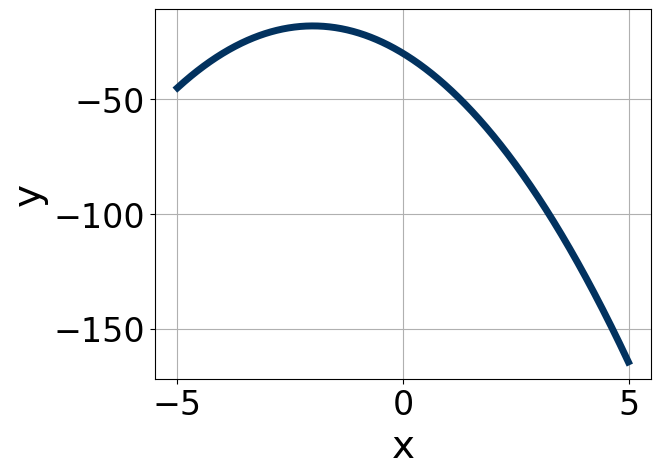
\includegraphics[width = 0.3\textwidth]{../Figures/quadraticEquationToGraphAA.png}\item 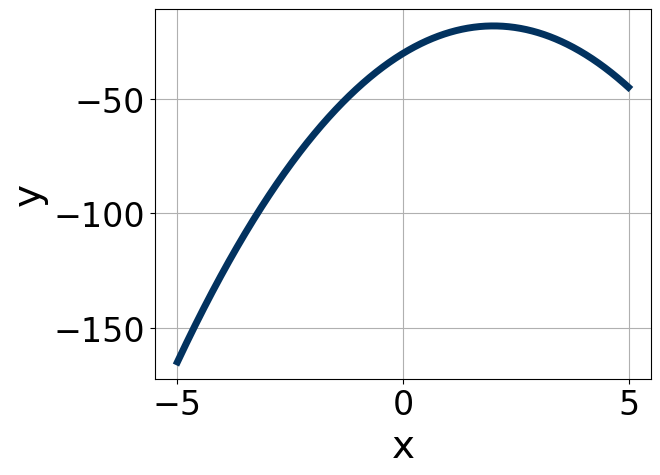
\includegraphics[width = 0.3\textwidth]{../Figures/quadraticEquationToGraphBA.png}\item 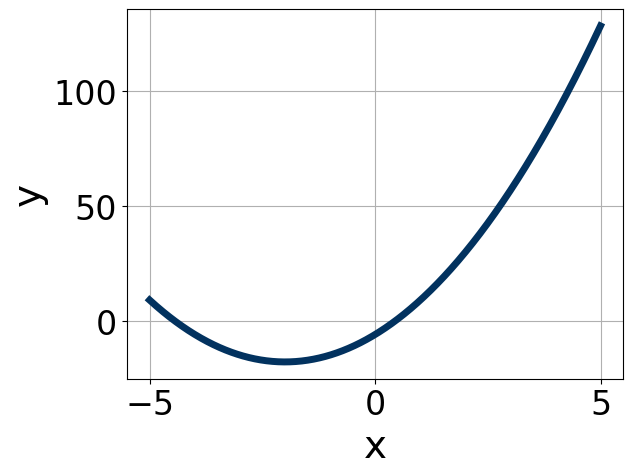
\includegraphics[width = 0.3\textwidth]{../Figures/quadraticEquationToGraphCA.png}\item 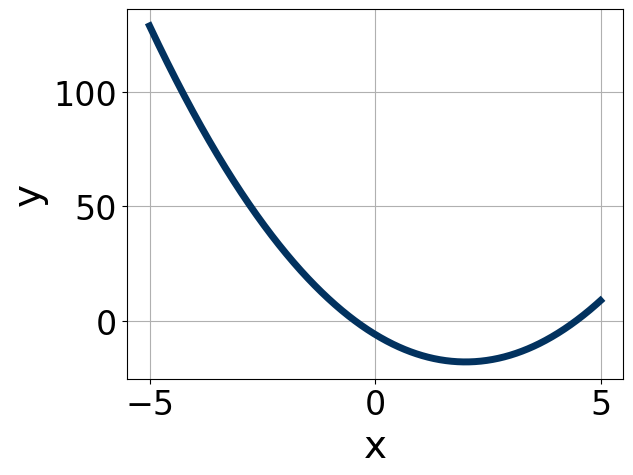
\includegraphics[width = 0.3\textwidth]{../Figures/quadraticEquationToGraphDA.png}\end{multicols}\item None of the above.
\end{enumerate} }
\litem{
Write the equation of the graph presented below in the form $f(x)=ax^2+bx+c$, assuming  $a=1$ or $a=-1$. Then, choose the intervals that $a, b,$ and $c$ belong to.
\begin{center}
    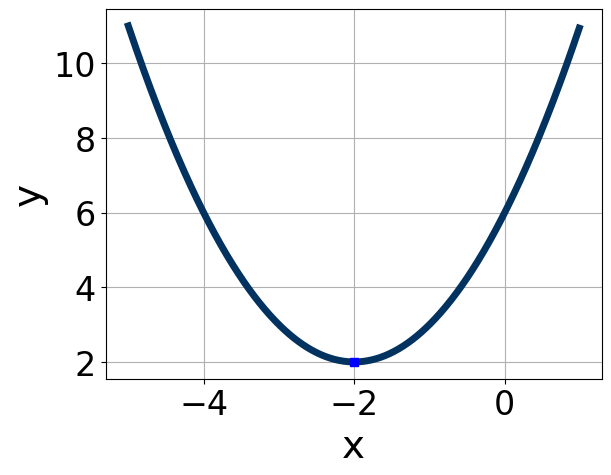
\includegraphics[width=0.5\textwidth]{../Figures/quadraticGraphToEquationA.png}
\end{center}
\begin{enumerate}[label=\Alph*.]
\item \( a \in [-1.7, -0.3], \hspace*{5mm} b \in [-5, -3], \text{ and } \hspace*{5mm} c \in [-2, 0] \)
\item \( a \in [-1.7, -0.3], \hspace*{5mm} b \in [-1, 7], \text{ and } \hspace*{5mm} c \in [-2, 0] \)
\item \( a \in [-0.5, 1.6], \hspace*{5mm} b \in [-5, -3], \text{ and } \hspace*{5mm} c \in [0, 5] \)
\item \( a \in [-0.5, 1.6], \hspace*{5mm} b \in [-5, -3], \text{ and } \hspace*{5mm} c \in [6, 7] \)
\item \( a \in [-0.5, 1.6], \hspace*{5mm} b \in [-1, 7], \text{ and } \hspace*{5mm} c \in [6, 7] \)

\end{enumerate} }
\litem{
Factor the quadratic below. Then, choose the intervals that contain the constants in the form $(ax+b)(cx+d); b \leq d.$\[ 54x^{2} -33 x -10 \]\begin{enumerate}[label=\Alph*.]
\item \( a \in [1.92, 2.94], \hspace*{5mm} b \in [-5, 0], \hspace*{5mm} c \in [24, 34], \text{ and } \hspace*{5mm} d \in [-1, 3] \)
\item \( a \in [0.57, 1.03], \hspace*{5mm} b \in [-49, -40], \hspace*{5mm} c \in [0, 2], \text{ and } \hspace*{5mm} d \in [9, 14] \)
\item \( a \in [11.87, 12.58], \hspace*{5mm} b \in [-5, 0], \hspace*{5mm} c \in [4, 5], \text{ and } \hspace*{5mm} d \in [-1, 3] \)
\item \( a \in [5.38, 6.08], \hspace*{5mm} b \in [-5, 0], \hspace*{5mm} c \in [7, 14], \text{ and } \hspace*{5mm} d \in [-1, 3] \)
\item \( \text{None of the above.} \)

\end{enumerate} }
\litem{
Solve the quadratic equation below. Then, choose the intervals that the solutions $x_1$ and $x_2$ belong to, with $x_1 \leq x_2$.\[ 25x^{2} +15 x -54 = 0 \]\begin{enumerate}[label=\Alph*.]
\item \( x_1 \in [-45.96, -44.18] \text{ and } x_2 \in [29.57, 30.1] \)
\item \( x_1 \in [-2.29, -1.39] \text{ and } x_2 \in [1.14, 1.28] \)
\item \( x_1 \in [-3.98, -3.12] \text{ and } x_2 \in [0.57, 0.64] \)
\item \( x_1 \in [-9.7, -8.02] \text{ and } x_2 \in [0.05, 0.25] \)
\item \( x_1 \in [-1.35, 0.14] \text{ and } x_2 \in [3.43, 3.76] \)

\end{enumerate} }
\litem{
Write the equation of the graph presented below in the form $f(x)=ax^2+bx+c$, assuming  $a=1$ or $a=-1$. Then, choose the intervals that $a, b,$ and $c$ belong to.
\begin{center}
    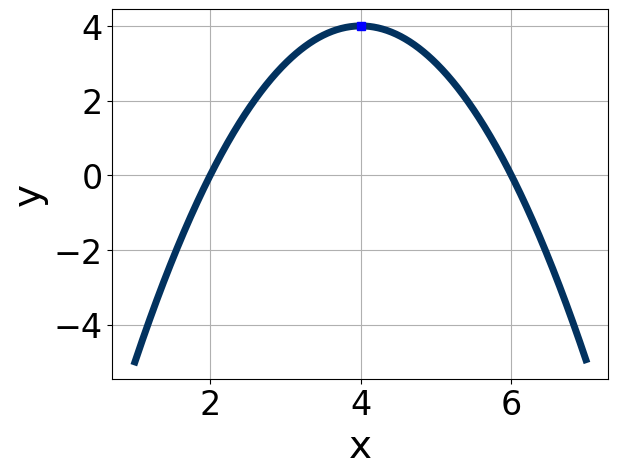
\includegraphics[width=0.5\textwidth]{../Figures/quadraticGraphToEquationCopyA.png}
\end{center}
\begin{enumerate}[label=\Alph*.]
\item \( a \in [-1, 0], \hspace*{5mm} b \in [7, 12], \text{ and } \hspace*{5mm} c \in [-14, -7] \)
\item \( a \in [-1, 0], \hspace*{5mm} b \in [-8, -4], \text{ and } \hspace*{5mm} c \in [-14, -7] \)
\item \( a \in [0, 5], \hspace*{5mm} b \in [7, 12], \text{ and } \hspace*{5mm} c \in [18, 22] \)
\item \( a \in [0, 5], \hspace*{5mm} b \in [-8, -4], \text{ and } \hspace*{5mm} c \in [18, 22] \)
\item \( a \in [-1, 0], \hspace*{5mm} b \in [-8, -4], \text{ and } \hspace*{5mm} c \in [-21, -17] \)

\end{enumerate} }
\litem{
Solve the quadratic equation below. Then, choose the intervals that the solutions belong to, with $x_1 \leq x_2$ (if they exist).\[ -18x^{2} +8 x + 2 = 0 \]\begin{enumerate}[label=\Alph*.]
\item \( x_1 \in [-0.3, 0] \text{ and } x_2 \in [0.47, 0.75] \)
\item \( x_1 \in [-0.9, -0.5] \text{ and } x_2 \in [-0.4, 0.4] \)
\item \( x_1 \in [-11.7, -10.7] \text{ and } x_2 \in [3.19, 3.82] \)
\item \( x_1 \in [-15.4, -13.3] \text{ and } x_2 \in [13.48, 14.68] \)
\item \( \text{There are no Real solutions.} \)

\end{enumerate} }
\litem{
Factor the quadratic below. Then, choose the intervals that contain the constants in the form $(ax+b)(cx+d); b \leq d.$\[ 16x^{2} +8 x -15 \]\begin{enumerate}[label=\Alph*.]
\item \( a \in [1.04, 3.02], \hspace*{5mm} b \in [-3, -1], \hspace*{5mm} c \in [7.36, 8.39], \text{ and } \hspace*{5mm} d \in [3, 8] \)
\item \( a \in [7.33, 9.11], \hspace*{5mm} b \in [-3, -1], \hspace*{5mm} c \in [1.17, 3.37], \text{ and } \hspace*{5mm} d \in [3, 8] \)
\item \( a \in [-0.67, 1.7], \hspace*{5mm} b \in [-15, -11], \hspace*{5mm} c \in [0.58, 1.89], \text{ and } \hspace*{5mm} d \in [20, 22] \)
\item \( a \in [2.63, 5.47], \hspace*{5mm} b \in [-3, -1], \hspace*{5mm} c \in [3.97, 5.28], \text{ and } \hspace*{5mm} d \in [3, 8] \)
\item \( \text{None of the above.} \)

\end{enumerate} }
\litem{
Graph the equation below.\[ f(x) = -(x+1)^2 - 13 \]\begin{enumerate}[label=\Alph*.]
\begin{multicols}{2}\item 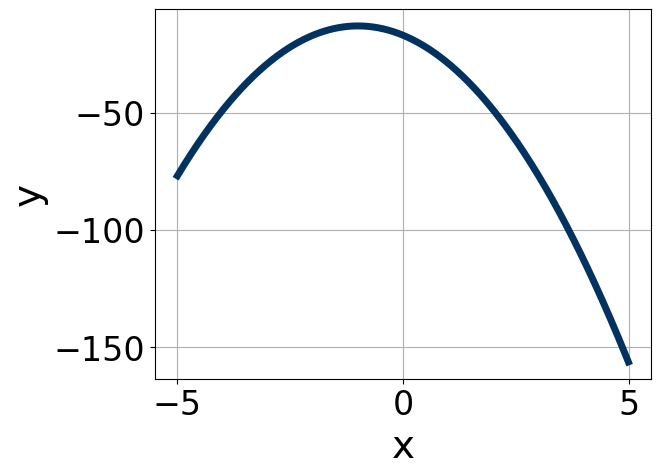
\includegraphics[width = 0.3\textwidth]{../Figures/quadraticEquationToGraphCopyAA.png}\item 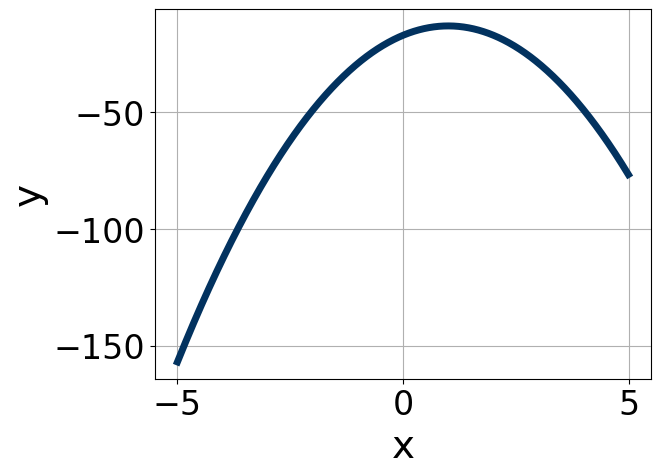
\includegraphics[width = 0.3\textwidth]{../Figures/quadraticEquationToGraphCopyBA.png}\item 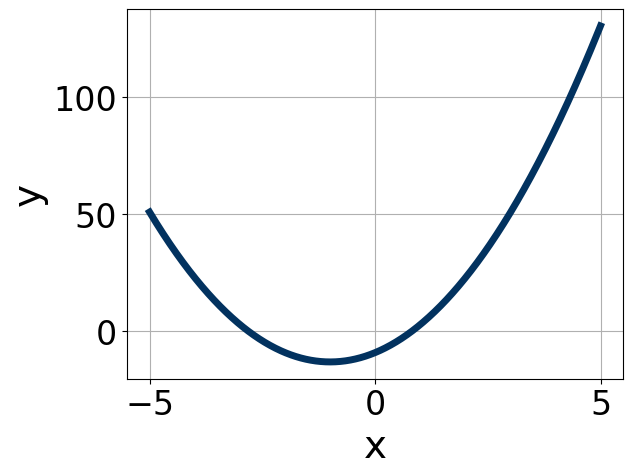
\includegraphics[width = 0.3\textwidth]{../Figures/quadraticEquationToGraphCopyCA.png}\item 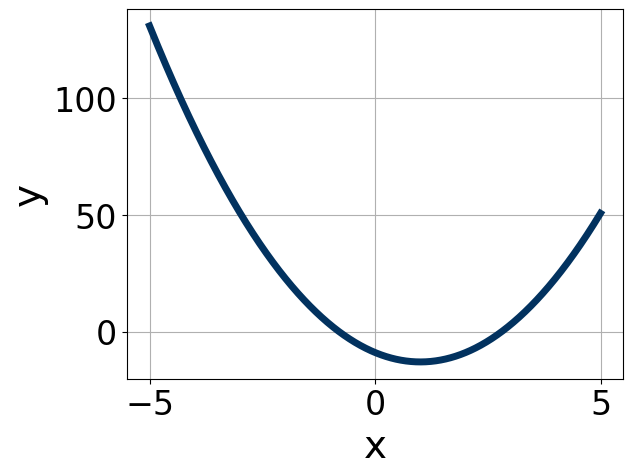
\includegraphics[width = 0.3\textwidth]{../Figures/quadraticEquationToGraphCopyDA.png}\end{multicols}\item None of the above.
\end{enumerate} }
\end{enumerate}

\end{document}